% Intended LaTeX compiler: pdflatex
\documentclass[12pt]{article}
\usepackage[utf8]{inputenc}
\usepackage[T1]{fontenc}
\usepackage{graphicx}
\usepackage{longtable}
\usepackage{wrapfig}
\usepackage{rotating}
\usepackage[normalem]{ulem}
\usepackage{amsmath}
\usepackage{amssymb}
\usepackage{capt-of}
\usepackage{hyperref}
\usepackage[english]{babel}
\usepackage{sbc-template}
\usepackage{url}
\sloppy
\renewcommand{\refname}{Referências}
\usepackage{algorithm}
\usepackage{algpseudocode}
\usepackage{xcolor}
\usepackage{listings}
\usepackage{booktabs}
\usepackage{url}
\usepackage{sbc-template}
\lstset{basicstyle=\footnotesize\ttfamily, frame=single, breaklines=true, numbers=left, numberstyle=\tiny\color{gray}, language=C, inputencoding=utf8, extendedchars=true}
\date{}
\title{Paralelização do Algoritmo Q-Learning com OpenMP}
\hypersetup{
 pdfauthor={Lucas Mello Schnorr},
 pdftitle={Paralelização do Algoritmo Q-Learning com OpenMP},
 pdfkeywords={},
 pdfsubject={},
 pdfcreator={Emacs 30.1 (Org mode 9.7.11)}, 
 pdflang={English}}
\begin{document}

\author{
   Rayan Raddatz de Matos (00584919) \inst{1},
   Eduardo Magnus Lazuta (00325091)\inst{1}, \\
   Enzo Lisbôa Peixoto (00584827)\inst{1}}

\address{
   Instituto de Informática, Universidade Federal do Rio Grande do Sul (UFRGS)\\
   Caixa Postal 15.064 -- 91.501-970 -- Porto Alegre -- RS -- Brazil
}

\maketitle
\section{Algoritmo e Problema}
\label{sec:orgcfa6d99}

O Q-Learning é um método de aprendizado por reforço que treina um
agente por meio de episódios. Em cada episódio, o agente parte do
estado inicial e executa ações até atingir o objetivo ou esgotar o
limite de passos. Cada passo atualiza a Q-Table com a equação de
Bellman: \(Q(s,a) \leftarrow Q(s,a) + \alpha[r + \gamma \max_{a'}
Q(s',a') - Q(s,a)]\). Após o treinamento, a política ótima é extraída
como \(\pi(s) = \arg\max_a Q(s,a)\).

O problema escolhido é pathfinding em grade \(L \times C\): o agente parte de
\((0,0)\) e deve atingir \((L{-}1,C{-}1)\) desviando de obstáculos com as
ações cima, baixo, esquerda, direita. Algoritmo \ref{alg:qlearning}
descrever o comportamento completo da aplicação sequencial.


\begin{algorithm}
\caption{Q-Learning Sequencial}
\label{alg:qlearning}
\begin{algorithmic}[1]
\Require Grid$(L, C)$, Obstáculos$(O)$, Episódios$(E)$, Max\_Passos$(P)$
\Require $\alpha$ (Aprendizado), $\gamma$ (Desconto), $\varepsilon$ (Exploração)
\Statex \textbf{1. INICIALIZAÇÃO E AMBIENTE}
\State Alocar dinamicamente $Q\_Table[\text{Estados}][\text{Ações}]$
\State Preencher $Q\_Table$ com zeros
\State Gerar Grid$(L, C)$ com Estado\_Inicial $s_0$ em $(0,0)$, Estado\_Objetivo $g$ em $(L{-}1, C{-}1)$
\State \hspace{1.5em} e posicionar $O$ obstáculos aleatórios (evitando $s_0$ e $g$)
\State Configurar Recompensas: $R_{\text{objetivo}}(+100)$, $R_{\text{obstáculo}}(-100)$, $R_{\text{passo}}(-1)$, $R_{\text{loop}}(-10)$
\Statex \textbf{2. NÚCLEO DE APRENDIZADO (Treinamento)}
\For{cada episódio de $1$ até $E$}
  \State $s \leftarrow s_0$ (Estado Inicial)
  \For{cada passo de $1$ até $P$}
    \State \textit{// Seleção de Ação ($\varepsilon$-Greedy)}
    \If{$\text{Random}(0, 1) < \varepsilon$}
      \State $a \leftarrow \text{Escolher\_Ação\_Aleatória()}$
    \Else
      \State $a \leftarrow \arg\max_{a'} Q[s][a']$ (Melhor ação conhecida)
    \EndIf
    \State \textit{// Interação com o Ambiente}
    \State $s' \leftarrow \text{Calcular\_Próximo\_Estado}(s, a)$
    \State $r \leftarrow \text{Avaliar\_Recompensa}(s')$
    \If{$s'$ já foi visitado neste episódio}
      \State $r \leftarrow r + R_{\text{loop}}$ \Comment{Penalidade de ciclo}
    \EndIf
    \State \textit{// Atualização de Bellman (Aprendizado Temporal)}
    \State $\text{Max\_Q\_Futuro} \leftarrow \text{Máximo}(Q[s'][\text{todas\_ações}])$
    \State $Q[s][a] \leftarrow Q[s][a] + \alpha \cdot (r + \gamma \cdot \text{Max\_Q\_Futuro} - Q[s][a])$
    \State \textit{// Transição de Estado}
    \State $s \leftarrow s'$
    \If{$s = g$}
      \State Encerrar Episódio (Objetivo Alcançado)
    \EndIf
  \EndFor
\EndFor
\Statex \textbf{3. PÓS-PROCESSAMENTO E SAÍDA}
\State Política\_Ótima $\pi(s) \leftarrow \arg\max_a Q[s][a]$
\State Imprimir Visualização do Grid com $\pi(s)$
\State Simular Caminho Final do Agente
\State Liberar Memória Alocada
\end{algorithmic}
\end{algorithm}
\section{Paralelização}
\label{sec:org36fb564}

\subsection{Escolha do Nível de Paralelismo}
\label{sec:orgf4b6894}

Quando paramos para discutir como paralelizar, tivemos três ideias:

\begin{itemize}
\item \textbf{Ações} (seleção do argmax): descartada, pois o número de ações é
apenas 4, o overhead de sincronização seria muito maior que qualquer
ganho.
\item \textbf{Steps} (passos dentro de um episódio): descartada, pois cada step depende
do estado resultante do passo anterior, dependência de dados
verdadeira faria com que as threads ficassem esperando e trabalhando
sequencialmente por baixo dos panos.
\item \textbf{Episódios}: escolhida. Episódios são independentes entre si: cada um parte
do estado inicial, executa uma trajetória completa e atualiza a Q-Table.
Não há dependência entre episódios distintos, o que permite distribuição
direta via \texttt{omp for}.
\end{itemize}


Após decidir começamos a paralelizar com o \texttt{omp parallel for},
entretanto após alguma execuções de teste vimos que apenas paralelizar
não seria o suficiente. Quando executamos vimos que nunca havia
convergência para o algoritmo paralelizado apesar de ter um grande
speedup. Isso acontecia pois ao rodar um problema com 10000 episódios
e 4 threads, por exemplo, cada thread executava 2500 episódios, mas
acabava por não comunicar seu conhecimento com as outras threads,
então o conhecimento final das 4 threads era o mesmo que rodar
sequencialmente com 2500 episódios, pensando nesse problema tivemos
que implementar sincronização ao código, limitando o potencial
paralelo.
\subsection{Sincronização no treino}
\label{sec:orgb346b31}

Cada thread mantém uma Q-Table local e executa um lote de episódios de
forma autônoma. Ao final de cada lote (\emph{chunk} de \texttt{sync\_interval}
episódios) as tabelas são fundidas na Q-Table global e
redistribuídas. O ciclo repete até esgotar os episódios:

\begin{lstlisting}[caption={Regiao paralela de train com sincronizacao (parallel\_qlearning\_cli.c)}]
#pragma omp parallel private(episode, state, action)
{
    int tid = omp_get_thread_num();
    QLearning local_ql  = *ql;
    local_ql.q_table    = local_q_tables[tid]; /* Q-Table propria por thread */
    local_ql.rand_seed  = cfg->seed + (unsigned int)tid;
    /* copia tabela global para local antes de comecar */
    #pragma omp barrier

    while (episode_start < cfg->num_episodes) {
        /* Treinamento local -- omp for distribui o chunk */
        #pragma omp for schedule(runtime)
        for (episode = episode_start; episode < episode_end; episode++)
            run_episode(&local_ql, episode);
        /* barreira implicita apos omp for */

        /* Merge com delta na Q-Table global */
        int active = (chunk_size < num_threads) ? chunk_size : num_threads;
        #pragma omp for collapse(2)
        for (state = 0; state < ql->num_states; state++)
            for (action = 0; action < NUM_ACTIONS; action++) {
                double snapshot  = ql->q_table[state][action];
                double delta_sum = 0.0;
                for (tt = 0; tt < num_threads; tt++)
                    delta_sum += local_q_tables[tt][state][action] - snapshot;
                ql->q_table[state][action] = snapshot + delta_sum / active;
            }

        /* Broadcast -- global copiada de volta para local */
        for (state ...) for (action ...)
            local_ql.q_table[state][action] = ql->q_table[state][action];
        #pragma omp barrier

        episode_start = episode_end;
    }
}
\end{lstlisting}

\textbf{Por que delta e não média absoluta?} Se um chunk tem menos episódios que
threads, algumas threads ficam ociosas e mantém \texttt{local\_ql.q\_table} igual
ao broadcast anterior (delta zero). Usar a média absoluta dividiria a soma dos
updates por \(T\) mesmo com apenas \(k < T\) threads ativas, diluindo o
aprendizado. O merge por delta divide apenas pelas \(k\) threads ativas
(\(\texttt{active} = \min(\texttt{chunk\_size}, T)\)), preservando o \(\alpha\)
efetivo de cada update.

\textbf{Heurísticas de \texttt{sync\_interval}}: foram implementadas duas estratégias
automáticas no dispatcher \texttt{train()}:

\begin{lstlisting}[caption={Calculo automatico do sync\_interval (train())}]
if (strcmp(cfg->sync_mode, "sqrt") == 0)
    /* sqrt(N/T): equilibra overhead de barreira e divergencia local */
    sync_interval = (int)sqrt((double)cfg->num_episodes / (double)num_threads);
else
    /* statespace: cada thread explora todos os estados antes de sincronizar */
    sync_interval = ql->num_states;   /* = L * C */
\end{lstlisting}

A heurística \texttt{sqrt} é inspirada em limites de \emph{regret} para SGD paralelo:
intervalos maiores aumentam a divergência entre tabelas locais; menores
aumentam o overhead das barreiras. A heurística \texttt{statespace} parte da
intuição de que cada thread deve visitar (em média) todos os estados do grid
uma vez antes de fundir o conhecimento, promovendo exploração mais
diversa. Além disso, testamos duas sincronizações fixas: a cada 10 episódios
e 1000 episódios.
\subsection{HOGWILD!}
\label{sec:orgde7dcd4}

Ao nos depararmos com o problema da sincronização, também buscamos se
existiam formas de fugir dela, nisso encontramos o algoritmo HOGWILD!
\cite{niu2011hogwild} . Ele elimina toda sincronização, nesse caso
todas as threads leem e escrevem na mesma Q-Table sem sincronização,
aceitando \emph{race conditions} intencionalmente. A implementação é minimal:

\begin{lstlisting}[caption={train\_hogwild com Q-Table compartilhada}]
#pragma omp parallel private(episode)
{
    int tid = omp_get_thread_num();

    /* Copia local apenas para rand_seed independente por thread.
     * importante: q_table herda o ponteiro da struct original ---
     * todas as threads leem/escrevem na mesma Q-Table sem nenhuma sincronizacao ou lock. */
    QLearning local_ql = *ql;
    local_ql.rand_seed = cfg->seed + (unsigned int)tid * 1000003U;

    #pragma omp for schedule(runtime)
    for (episode = 0; episode < cfg->num_episodes; episode++)
        run_episode(&local_ql, episode);   /* le/escreve shared sem lock */
}
\end{lstlisting}

 o ponteiro é copiado por valor, continuando a apontar para a Q-Table
original compartilhada. Apenas \texttt{rand\_seed} é isolado por thread,
garantindo trajetórias distintas sem overhead de sincronização.

Três propriedades do problema justificam a corretude prática do método:

\begin{itemize}
\item \textbf{Esparsidade}: cada episódio visita uma fração pequena dos \(L \times C\)
estados; conflitos simultâneos em \(Q(s,a)\) são raros.
\item \textbf{Escala dos updates}: cada atualização é ponderada por \(\alpha \leq 0{,}1\);
sobrescrever um update ocasional é um ruído de ordem \(O(\alpha)\),
desprezível para a convergência.
\item \textbf{Simetria direcional}: ambos os valores concorrentes são gradientes válidos
calculados de trajetórias distintas; nenhum é incorreto.
\end{itemize}

Importante notar que nesse caso, quanto mais esparsa a entrada, no
nosso caso, quanto mais estados existirem, melhor performará o algoritmo.
\section{Metodologia Experimental}
\label{sec:org53b1e5b}

O experimento adota um design fatorial completo sobre os fatores
listados na Tabela \ref{tab:org8f369ab}. Para cada combinação de
parâmetros, o tempo de treinamento (medido dentro de \texttt{train()}) é
registrado em múltiplos blocos de replicação, permitindo estimar a
variância de tempo devida ao escalonador do sistema operacional.

\begin{table}[htbp]
\caption{\label{tab:org8f369ab}Fatores e níveis do experimento.}
\centering
\small
\begin{tabular}{lp{3.5cm}p{6cm}}
\toprule
Fator & Níveis & Motivação\\
\midrule
Threads & 1, 2, 4, 8, 16, 20, 40 & Cobre desde serial até hyperthreading completo\\
Tamanho do grid & 10, 50, 100 & Espaço de estados pequeno, médio e grande\\
Modo de sync & \texttt{sqrt}, \texttt{statespace}, \texttt{hogwild} & Três estratégias de paralelização\\
Episódios & 5000, 10000 & Limiar de convergência: 5k instável, 10k estável\\
Densidade obst. & 0\%, 50\% & Grid livre vs. grade com alta densidade\\
Schedule OpenMP & \texttt{static}, \texttt{guided}, \texttt{dynamic} & Políticas de distribuição de trabalho\\
Chunk & 0, 1, 10 & Granularidade do chunking para modo \texttt{guided/dynamic}\\
 &  & \\
\bottomrule
\end{tabular}
\end{table}
\subsection{Baseline Sequencial}
\label{sec:org9168f76}

Linhas com \texttt{threads=1} invocam o binário sequencial puro, sem runtime
OpenMP. Isso garante que o speedup seja calculado contra o tempo real
do algoritmo, sem incluir o overhead de criação do pool de threads do
OpenMP no denominador.
\subsection{Afinidade de Threads}
\label{sec:orgd70a030}

Importante notar que adotamos a política de afinidade de acordo com o número de threads:

\begin{itemize}
\item \(T \leq 20\): \texttt{OMP\_PLACES=cores}, \texttt{OMP\_PROC\_BIND=close}, uma thread
por núcleo físico, sem hyperthreading, minimizando contenção de cache.
\item \(T = 40\): \texttt{OMP\_PLACES=threads}, \texttt{OMP\_PROC\_BIND=close}, uma thread
por CPU lógica, utilizando hyperthreading completo.
\end{itemize}
\subsection{Medição de Tempo}
\label{sec:org1b36bdc}

O tempo registrado em \texttt{training\_time\_s} corresponde exclusivamente à
execução de \texttt{train()}, excluindo inicialização do ambiente, alocação de
memória e impressão de resultados. O binário paralelo usa
\texttt{omp\_get\_wtime()} e o sequencial usa \texttt{clock\_gettime(CLOCK\_MONOTONIC)},
ambos medindo tempo de parede (\emph{wall-clock}). Também foi pega o tempo do
VTUNE, entretanto não foi utilizado por demonstrar uma variabilidade
muito maior.
\section{Resultados}
\label{sec:org3e8794b}
\subsection{Speedup e Eficiência}
\label{sec:org3234da1}

O speedup médio por número de threads e modo de sincronização está
apresentado na Figura \ref{fig:orgb75c4f7}. O eixo tracejado representa
o speedup ideal (linear). Para grids 10x10, o speedup satura rapidamente
em torno de 4--5x a partir de 8 threads, indicando que o trabalho por
thread é insuficiente para amortizar o overhead de sincronização. Para
grids maiores (100x100), o HOGWILD! atinge speedup médio de até 17x com
40 threads, enquanto os modos com sincronização (\textit{sqrt},
\textit{statespace}) ficam abaixo de 10x. A diferença se deve ao fato de
que os modos sincronizados impõem barreiras periódicas que serializam
parcialmente a execução.

\begin{figure}[htbp]
\centering
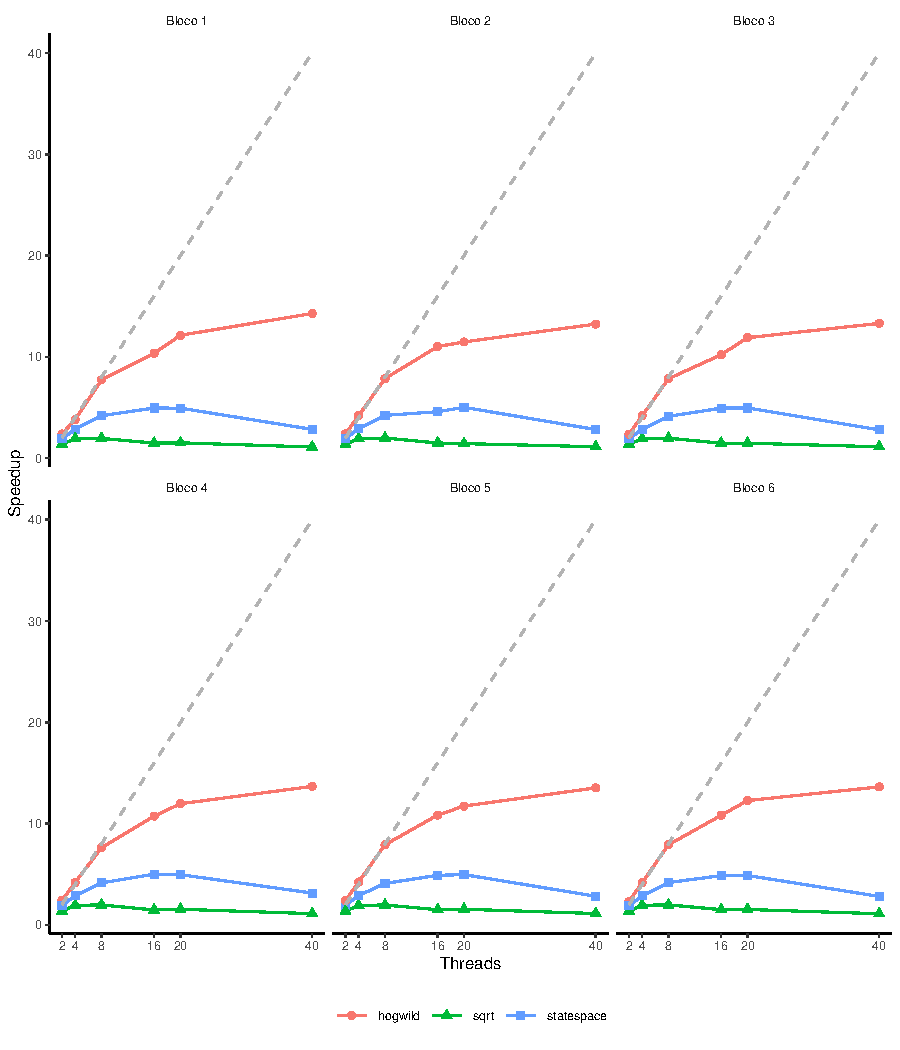
\includegraphics[width=.9\linewidth]{speedup_blocks.pdf}
\caption{\label{fig:orgb75c4f7}Speedup médio por modo de sincronização (10k episódios). Tracejado = ideal linear.}
\end{figure}

A eficiência paralela (\(S(T)/T\)) é mostrada na Figura \ref{fig:org8213673}.
No grid 10x10, vários modos apresentam eficiência acima de 100\%,
possivelmente por efeitos de cache com múltiplos núcleos acessando
partições distintas da Q-Table. Ainda assim, a eficiência colapsa
rapidamente: nenhuma configuração sustenta 50\% além de 8 threads neste
grid, resultado consistente com o tráfego de coerência de cache
discutido na Seção de Análise de Cache.

Para grids maiores, o HOGWILD! mantém a melhor eficiência em todos os
tamanhos: cerca de 35--45\% com 40 threads no grid 100x100, enquanto
os demais modos ficam abaixo de 15\%. Entre os modos sincronizados,
o \textit{every10} (sincronização a cada 10 episódios) apresenta a pior
eficiência. O overhead de barreiras frequentes supera o ganho da
convergência mais rápida. O \textit{every1000} e o \textit{statespace}
mantêm eficiência intermediária, pois sincronizam com menos frequência
e amortizam o custo das barreiras sobre mais trabalho útil.

\begin{figure}[htbp]
\centering
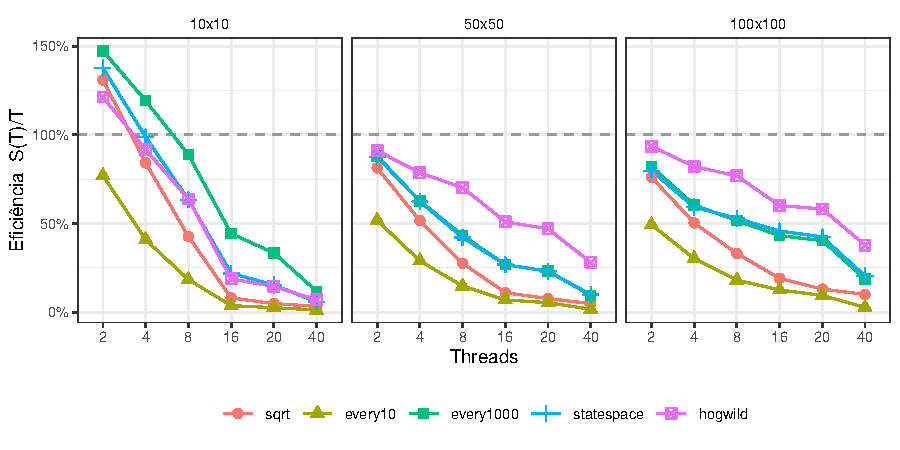
\includegraphics[width=.9\linewidth]{efficiency.pdf}
\caption{\label{fig:org8213673}Eficiência paralela por modo de sincronização (10k episódios). Ideal = 100\% (tracejado).}
\end{figure}
\subsection{Análise de Cache (10x10)}
\label{sec:org9fe480c}

Uma coisa que procuramos entender mais a fundo foi a perda do speedup
no grid 10x10 após 8 threads. Para isso usamos o \texttt{perf stat} (eventos
\texttt{L1-dcache-load-misses}, \texttt{LLC-loads} e \texttt{LLC-load-misses}) para todas as
combinações de sync-mode e schedule com 10k episódios pois o vtune
apresentou erros de versão. A Q-Table do grid 10x10 ocupa apenas 3,2 KB
(100 estados \(\times\) 4 ações \(\times\) 8 bytes), cabendo inteiramente em L1
(32 KB). O baseline sequencial confirma isso com apenas 0,18\% de
L1-miss.

\begin{table}[htbp]
\caption{\label{tab:org0317c3a}L1-miss e LLC-miss por threads e modo de sync (media dos tres schedules, grid 10x10, 10k ep.).}
\centering
\small
\begin{tabular}{rrrrrrr}
\toprule
Threads & sq-L1 & sq-LLC & spc-L1 & spc-LLC & hog-L1 & hog-LLC\\
\midrule
2 & 1,12\% & 0,80\% & 1,10\% & 1,11\% & 7,42\% & 0,44\%\\
4 & 3,87\% & 0,70\% & 4,10\% & 0,79\% & 8,53\% & 0,18\%\\
8 & 6,37\% & 0,17\% & 5,15\% & 0,18\% & 23,20\% & 0,11\%\\
\midrule
16 & 3,95\% & 30,9\% & 4,64\% & 23,1\% & 5,99\% & 36,7\%\\
20 & 5,08\% & 29,1\% & 11,09\% & 22,9\% & 1,38\% & 36,4\%\\
40 & 1,99\% & 40,7\% & 1,98\% & 28,5\% & 4,17\% & 35,9\%\\
\bottomrule
\end{tabular}
\end{table}

As máquinas hype tem um dual-socket (2x Intel Xeon E5-2650 v3, 10
núcleos por socket). Com \texttt{OMP\_PLACES=cores} e \texttt{OMP\_PROC\_BIND=close}, os
threads são alocados em núcleos consecutivos: \(T \leq 10\) ficam
inteiramente no socket\textasciitilde{}0; \(T = 16\) já usa 10 núcleos do socket\textasciitilde{}0 e 6
do socket\textasciitilde{}1.

Para \(T \leq 8\), hogwild apresenta L1-miss elevado (7--23\%) mas LLC-miss
abaixo de 0,5\% (Tabela \ref{tab:org0317c3a}): cada escrita na Q-Table compartilhada
invalida a linha de cache nos demais núcleos, forçando recargas de
L2/L3, mas os dados são encontrados antes do LLC. Os modos
sincronizados (sqrt, statespace) mantêm L1-miss baixo (\(\leq 6,4\%\)) pois
cada thread opera em cópia local sem invalidações.

A partir de \(T = 16\), threads do socket 1 passam a acessar a Q-Table
alocada na memória do socket 0 para o hogwild. O que aparece como
LLC-miss no L3 local do socket 1. Para o hogwild esse custo é pago em
cada acesso, pois não há cópia local: daí os 36,7\% de LLC-miss.  Para
statespace, os threads do socket 1 carregam a cópia local uma vez e a
reutilizam por 100 episódios antes do próximo merge, amortizando os
misses e chegando a apenas 23,1\%.

Em todos os modos, a fronteira entre socket 0 e socket 1 é o ponto de
ruptura do LLC-miss, confirmando que o gargalo do grid 10x10 com
muitas threads é tráfego de cache, não escassez de
trabalho por thread.
\subsection{Análise de Cache (100x100)}
\label{sec:orgc84981b}

A Q-Table do grid 100x100 ocupa 320 KB (\(10^4\) estados \(\times\) 4 ações
\(\times\) 8 bytes), excedendo o L1 (32 KB) e o L2 (\(\approx\)256 KB) mas
cabendo no LLC (20 MB). O baseline sequencial já exibe 2,82\%
de L1-miss (vs. 0,18\% no grid 10x10), confirmando que a tabela
transborda o L1 desde o início.

\begin{table}[htbp]
\caption{\label{tab:org04378e1}L1-miss e LLC-miss por threads e modo de sync (media dos tres schedules, grid 100x100, 10k ep.).}
\centering
\scriptsize
\begin{tabular}{rrrrrrrrr}
\toprule
Threads & sq-L1 & sq-LLC & ev1k-L1 & ev1k-LLC & spc-L1 & spc-LLC & hog-L1 & hog-LLC\\
\midrule
2 & 5,63\% & 0,06\% & 3,39\% & 0,08\% & 3,28\% & 0,08\% & 4,50\% & 0,00\%\\
4 & 6,27\% & 0,12\% & 2,91\% & 0,29\% & 2,62\% & 0,05\% & 4,30\% & 0,00\%\\
8 & 7,80\% & 0,01\% & 2,64\% & 0,04\% & 2,09\% & 0,05\% & 5,41\% & 0,20\%\\
\midrule
16 & 11,79\% & 7,01\% & 1,98\% & 3,12\% & 2,18\% & 1,59\% & 4,36\% & 35,44\%\\
20 & 12,85\% & 22,43\% & 2,83\% & 14,03\% & 2,17\% & 5,43\% & 3,78\% & 33,49\%\\
40 & 11,03\% & 27,65\% & 3,01\% & 16,47\% & 2,01\% & 2,61\% & 2,56\% & 60,77\%\\
\bottomrule
\end{tabular}
\end{table}

Para \(T \leq 8\), o LLC-miss permanece abaixo de 0,3\% em todos os
modos (Tabela \ref{tab:org04378e1}): a Q-Table inteira cabe no LLC e cada thread
opera em sua cópia local sem competição inter-socket. A partir de \(T =
16\) os comportamentos divergem:

\begin{itemize}
\item \textbf{Hogwild} atinge 35,4\% de LLC-miss com 16 threads e 60,8\% com 40.
A única Q-Table de 320 KB é escrita continuamente por todos os
threads, invalidando linhas.
\item \textbf{Statespace} chega a apenas 2,6\% com 40 threads. O intervalo de
sincronização é igual ao número de estados (\(10^4\) episódios para o
grid 100x100), resultando em uma única sincronização durante o
treino.
\item \textbf{Every1000} (16,5\% com 40 threads) fica entre sqrt e statespace:
sincroniza a cada 1000 episódios, menos frequente que o heurístico
sqrt (27,7\%).
\end{itemize}

No eixo de L1-miss, every10 (não incluído na tabela) alcança 10--15\%
em todos os níveis de threads por copiar os 320 KB da Q-Table a cada
10 episódios, expulsando dados úteis do L1 repetidamente. Os demais
modos ficam entre 2--13\%, reflexo direto de quão frequentemente o
merge copia a tabela inteira.

Diferente do grid 10x10 onde o L1-miss é desprezível e o gargalo
aparece de forma abrupta no LLC a partir de \(T = 16\), no grid
100x100 o L1-miss já é estrutural e o LLC-miss reflete diretamente a
frequência de sincronização: intervalos curtos geram mais tráfego de
coerência, intervalos longos preservam a localidade.
\subsection{Análise VTune}
\label{sec:orgc9ac33c}

O Intel VTune Profiler foi utilizado no modo \textit{performance-snapshot}
para coletar IPC (\textit{Instructions Per Cycle}) e percentual de
\textit{Memory Bound} por configuração (Figura \ref{fig:orgc15a476}).

\begin{figure}[htbp]
\centering
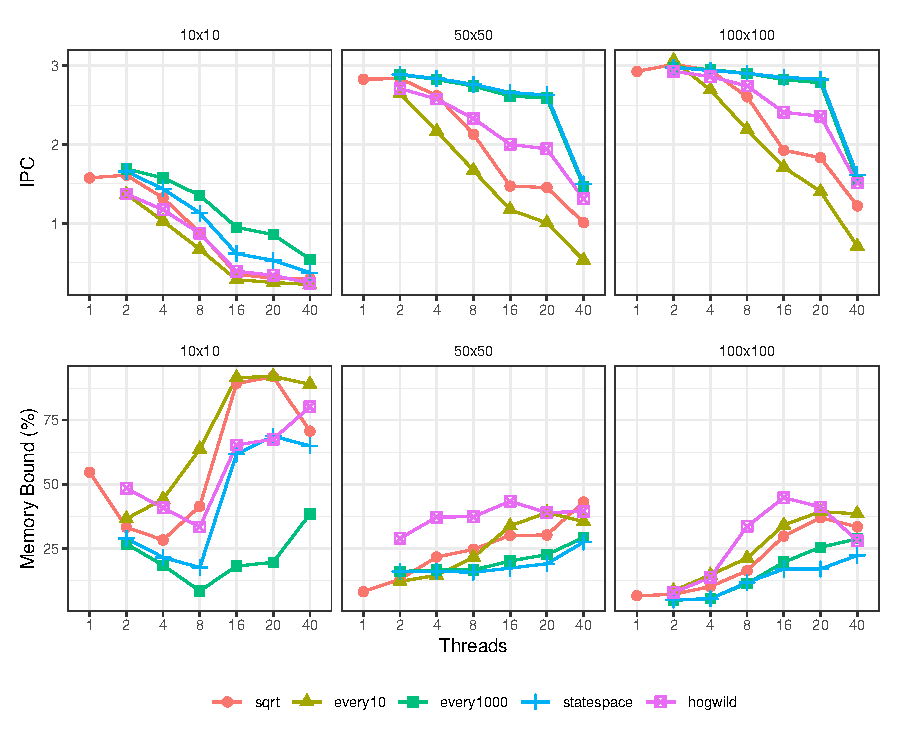
\includegraphics[width=.9\linewidth]{vtune.pdf}
\caption{\label{fig:orgc15a476}IPC (topo) e Memory Bound \% (baixo) por modo de sincronização e tamanho de grid.}
\end{figure}

IPC decai com o número de threads em todos os cenários. Isso é
esperado pois IPC mede eficiência de execução por thread, e mais
threads aumentam a contenção por cache e barramento sem aumentar o
throughput individual. Além disso, ao ativar o hyperthreading, dois
threads lógicos compartilham o mesmo núcleo físico, pressionando ainda
mais a cache. O conjunto de linhas de cache ativas dobra sem aumentar
a capacidade do L1. Ainda no tópico do grid 10x10, vemos um alto
Memory Bound e baixo IPC, reforçando o que foi visto na análise das
cache. Esse tamanho faz com que múltiplas threads atualizem um
conjunto muito restrito de linhas de cache com alta frequência.
\subsection{Análise de fatores de menor impacto}
\label{sec:org1c26d1b}

Além do modo de sincronização, o experimento variou o schedule do
OpenMP (static, dynamic, guided), o tamanho de chunk (auto, 1, 10) e a
densidade de obstáculos (0\%, 50\%). Os efeitos desses fatores concretos
no tempo de execução e speedup não foi significativo. Os efeitos são
analisados abaixo para o grid 100x100 com 10k episódios.

\textbf{Schedule e chunk.} A Figura \ref{fig:org7f7cda0} mostra o speedup médio por
schedule, separado por tamanho de chunk e grid. Os três schedules
produzem speedup praticamente idêntico: as durações de episódio são
homogêneas e qualquer distribuição de carga é equilibrada. A diferença
geral permanece pequena (<2\% no speedup médio), indicando que o
schedule não é o fator dominante. O chunk tem impacto igualmente
pequeno.

\begin{figure}[htbp]
\centering
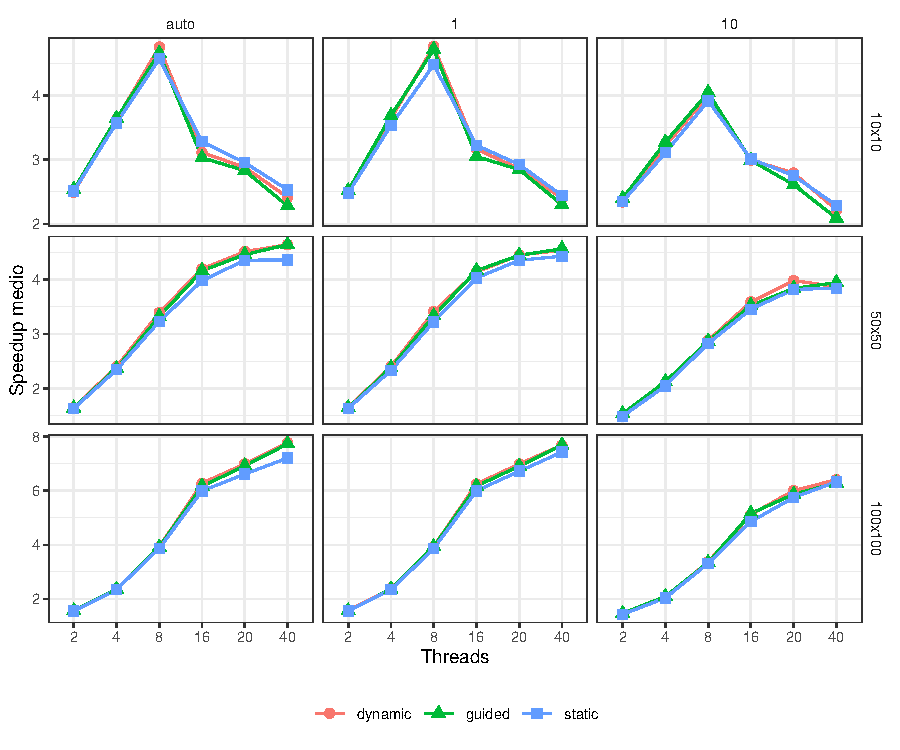
\includegraphics[width=.9\linewidth]{sched_impact.pdf}
\caption{\label{fig:org7f7cda0}Speedup medio por schedule, separado por chunk e grid (10k ep., media sobre obstacles e sync-mode).}
\end{figure}

\textbf{Densidade de obstáculos.} A Figura \ref{fig:orgfc1e46e} mostra o
tempo de treinamento absoluto para 0\% e 50\% de obstáculos. Com 50\%
de obstáculos, o agente nunca encontra o objetivo e cada episódio
percorre todos os \texttt{max\_steps} passos, tornando o tempo sequencial
muito maior. É importante notar que comparar speedup entre as duas
densidades seria injusto: o ganho aparente com 50\% de obstáculos
reflete apenas que há mais trabalho total a dividir entre as threads
--- não que o algoritmo paralelo seja mais eficiente. O gráfico de
tempo absoluto deixa claro que ambas as versões (0\% e 50\%) escalam
de forma semelhante com mais threads, mas partem de baselines
completamente diferentes.

\begin{figure}[htbp]
\centering
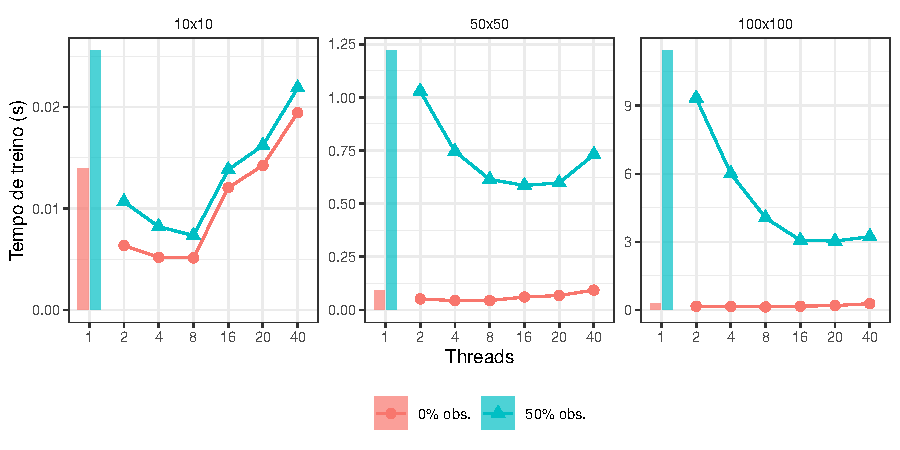
\includegraphics[width=.9\linewidth]{obs_speedup.pdf}
\caption{\label{fig:orgfc1e46e}Tempo de treino por densidade de obstáculos (10k ep., media sobre configs e schedules). Barra = sequencial (1 thread), linhas = paralelo.}
\end{figure}
\subsection{Convergência}
\label{sec:orgb21221d}

A Figura \ref{fig:orga7a727c} apresenta a taxa de convergência em função
do número de threads, separada por densidade de obstáculos, para o grid
100x100 com 10k episódios. Com 0\% de obstáculos, todos os modos
convergem razoavelmente para poucos threads, mas degradam com o aumento
do paralelismo. Com 50\% de obstáculos, com exceção do pequeno grid
10x10, nenhum dos outros convergiu.

\begin{figure}[htbp]
\centering
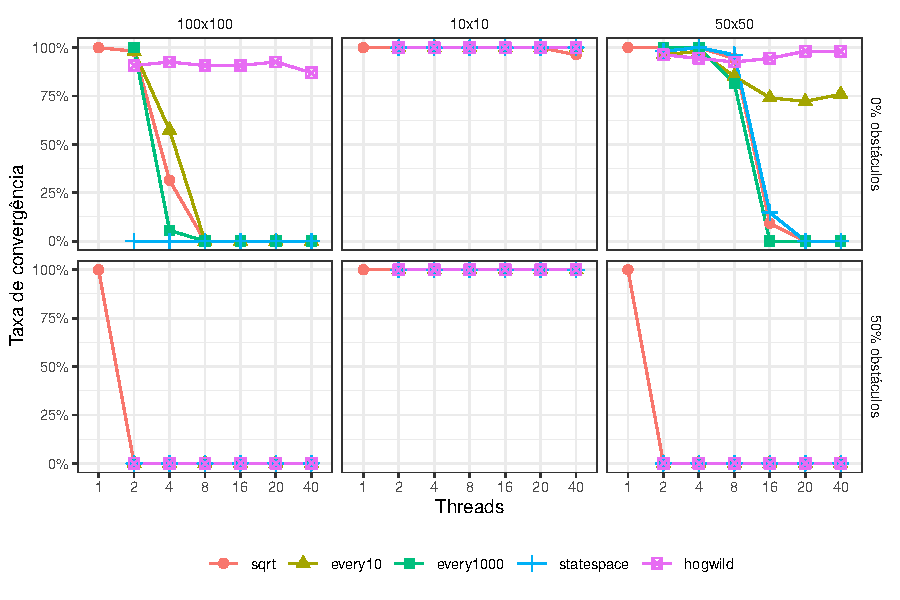
\includegraphics[width=.9\linewidth]{conv_obstacles.pdf}
\caption{\label{fig:orga7a727c}Taxa de convergência por modo de sincronização e densidade de obstáculos (10k ep.).}
\end{figure}

A causa da degradação nos modos sincronizados é a \textbf\{divisão de
episódios\}: com \(T\) threads e \(E\) episódios totais, cada thread treina
com apenas \(E/T\) episódios. Quando \(E/T\) cai abaixo do limiar mínimo de
convergência \(E_{\min}\) do problema, o agente não acumula experiência
suficiente para aprender uma política válida. Esse limiar é mais alto
com 50\% de obstáculos, pois o agente precisa explorar trajetórias mais
longas até encontrar o objetivo, exigindo mais episódios para propagar
valores Q corretos a todos os estados relevantes.

Mesmo o HOGWILD! usando uma Q-Table compartilhada, que em teoria
acumula atualizações de \textit{todos} os threads simultaneamente não
foi capaz de convergir nesses casos com muitos obstáculos. Isso nos
diz que apenas uma boa heurística não é o suficiente para o problema
convergir, também é necessário aumentar o tamanho do problema.
\subsection{Speedup das Configurações Convergidas}
\label{sec:orgcf56a85}

A tabela a seguir apresenta o speedup médio considerando apenas as
execuções que convergiram (10k episódios). Células vazias indicam que
nenhuma execução da combinação convergiu.

\begin{table}

\caption{Speedup medio apenas para execucoes convergidas (10k episodios). Celulas vazias: nenhuma execucao convergiu nessa combinacao.}
\centering
\begin{tabular}[t]{llrrrrrr}
\toprule
Grid & Config & 2 & 4 & 8 & 16 & 20 & 40\\
\midrule
10x10 & sqrt & 2.62 & 3.37 & 3.42 & 1.29 & 0.97 & 1.32\\
10x10 & every10 & 1.54 & 1.63 & 1.47 & 0.59 & 0.51 & 0.49\\
10x10 & every1000 & 2.95 & 4.77 & 7.11 & 7.09 & 6.69 & 4.73\\
10x10 & statespace & 2.75 & 3.95 & 5.07 & 3.51 & 3.07 & 2.34\\
10x10 & hogwild & 2.43 & 3.67 & 5.11 & 3.00 & 2.91 & 2.78\\
50x50 & sqrt & 1.98 & 2.33 & 2.20 & 1.19 & NA & NA\\
50x50 & every10 & 1.08 & 1.11 & 0.98 & 0.65 & 0.59 & 0.38\\
50x50 & every1000 & 2.21 & 2.96 & 3.76 & NA & NA & NA\\
50x50 & statespace & 2.20 & 2.91 & 3.58 & 4.16 & NA & NA\\
50x50 & hogwild & 2.32 & 4.04 & 7.40 & 9.19 & 10.12 & 10.65\\
100x100 & sqrt & 1.77 & 1.99 & NA & NA & NA & NA\\
100x100 & every10 & 0.90 & 0.85 & NA & NA & NA & NA\\
100x100 & every1000 & 1.97 & 2.49 & NA & NA & NA & NA\\
100x100 & hogwild & 2.43 & 4.24 & 8.00 & 11.45 & 13.88 & 18.14\\
\bottomrule
\end{tabular}
\end{table}
\section{Conclusão}
\label{sec:org32001cc}

Este trabalho paralelizou o Q-Learning por episódios usando OpenMP com
diferentes estratégias e heurísticas.

O principal limitante de convergência identificado foi a divisão de
episódios. com \(T\) threads e \(E\) episódios fixos, cada thread treina
com apenas \(E/T\) episódios. Quando esse valor cai abaixo do limiar
mínimo do problema, o agente não aprende uma política válida. A
sincronização e as heurísticas selecionadas conseguem fazer o cenário
ficar favorável, mas ainda não garantem precisão. Com 50\% de
obstáculos, nenhuma configuração paralela convergiu para mapas
"grandes", incluindo o HOGWILD!, que embora acumule updates de todas
as threads, sofre com race conditions que corrompem o aprendizado em
ambientes densos.

Em grids pequenos (10x10), o gargalo é diferente: a Q-Table cabe em
L1, mas com grande quantidade de threads, ocorrem invalidações de
coerência de cache que saturam o LLC e degradam IPC e speedup
independentemente do modo de sincronização.

O HOGWILD! obteve o maior speedup bruto (até 17x com 40 threads em
grids grandes), beneficiando-se da ausência de barreiras e do acesso
esparso à Q-Table em grids 100x100. Os modos sincronizados com
intervalos longos (every1000, statespace) mostraram
melhor comportamento de cache por manter Q-Tables locais isoladas por
mais tempo entre syncs, mas demonstrarão pior conversão.

O benefício prático do paralelismo está na redução do tempo de
treinamento para um orçamento fixo de episódios, em cenários onde esse
orçamento dividido é suficiente para o tamanho e complexidade do
problema.
\bibliographystyle{sbc.bst}
\bibliography{refs}
\end{document}
